\begin{center}
\begin{minipage}{\linewidth}\centering
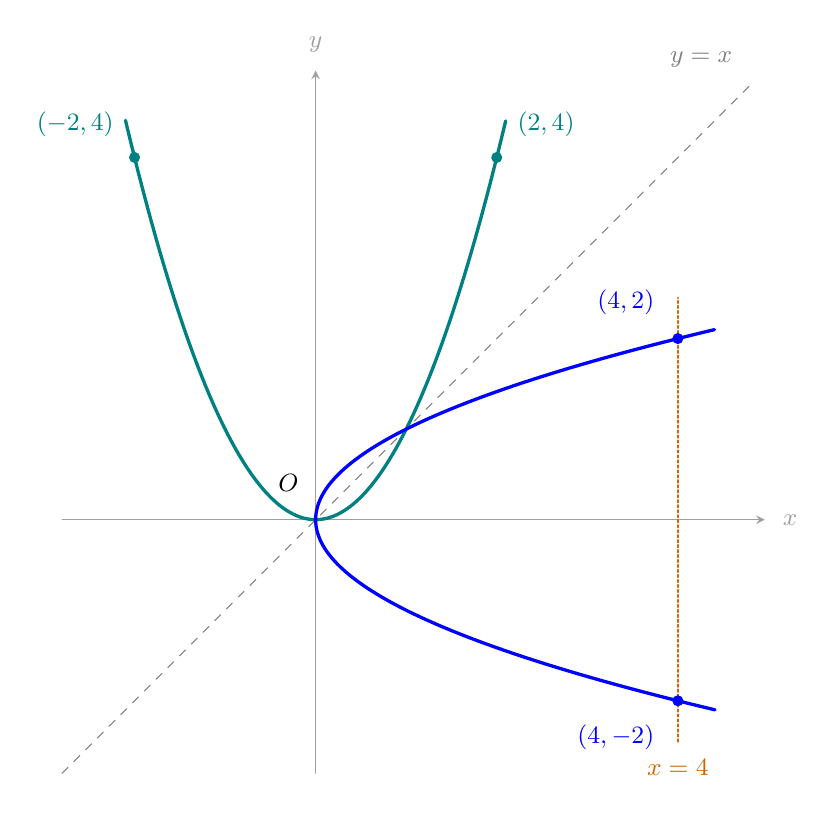
\begin{tikzpicture}[x=1.15cm,y=1.15cm,>=stealth,font=\small,line cap=round,line join=round]
\draw[->,gray!75] (-2.8,0)--(4.96,0) node[right=3pt]{$x$};
\draw[->,gray!75] (0,-2.8)--(0,4.96) node[above=3pt]{$y$};
\node at (-.3,.4) {$O$};
\draw[gray,dashed] (-2.8,-2.8)--(4.8,4.8) node[above left=3pt]{$y=x$};

\draw[teal,very thick,domain=-2.1:2.1,samples=121] plot(\x,{\x*\x});
\draw[blue,very thick,domain=-2.1:2.1,samples=121] plot({\x*\x},\x);
\draw[orange!80!black,densely dotted,thick] (4,-2.45)--(4,2.45);
\node[orange!80!black,below=3pt] at (4,-2.45) {$x=4$};
\fill[blue] (4,2) circle(2pt) node[above left=5pt]{$(4,2)$};
\fill[blue] (4,-2) circle(2pt) node[below left=5pt]{$(4,-2)$};
\fill[teal] (-2,4) circle(2pt) node[above left=4pt]{$(-2,4)$};
\fill[teal] (2,4) circle(2pt) node[above right=4pt]{$(2,4)$};

\end{tikzpicture}\par\smallskip
{\small \textcolor{teal}{\rule[.5ex]{1em}{.8pt}\ $y=x^2,\ x\in\mathbb R$}\qquad\textcolor{blue}{\rule[.5ex]{1em}{.8pt}\ $x=y^2$（镜像关系）}}\par
{\small 镜像在同一输入 $4$ 处有两个输出 $\pm2$，不能整体写成反函数。}\par\smallskip
\end{minipage}
\end{center}
